\section{Overview} \label{sec:overview}

\subsection{\xxx Work Flow}

\begin{figure*}[tb]
    \centering
    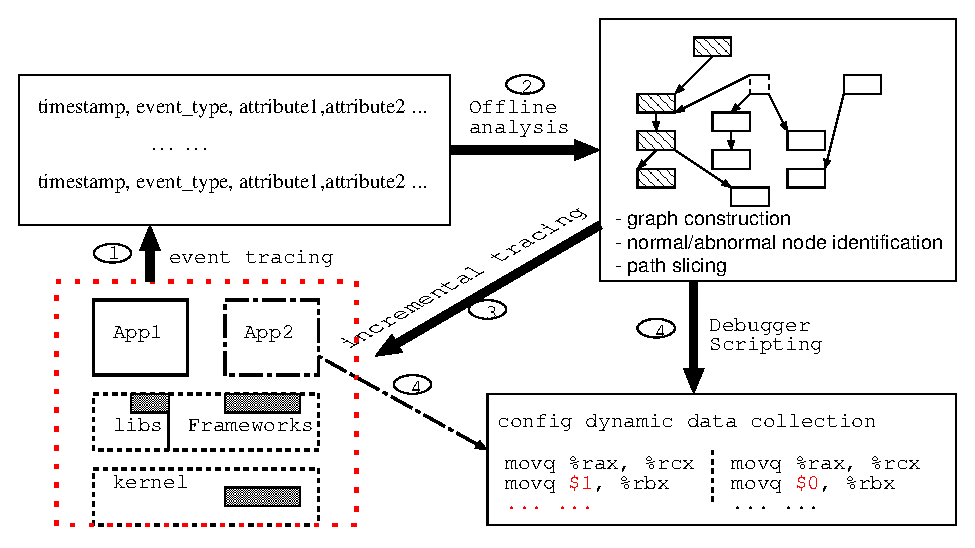
\includegraphics[width=0.8\linewidth]{ArgusOverview.eps}
    \caption{\xxx Work Flow}
    \label{fig:argus-overview}
\end{figure*}

Figure~\ref{fig:argus-overview} shows \xxx's work flow, which consists of two
phases.  A user runs command ``\v{\xxx start}'' to enter the system-wide
tracing phase, within which \xxx logs events including system calls,
inter-process communications (IPCs), and waits and wake-ups from all
applications and daemons.  Occasionally based on user configurations, it logs
data flag accesses leveraging hardware watch-point registers.  Each log entry
includes a timestamp, the event type, key attributes of the event, and a
lightweight call stack obtained by unwinding the stack pointer.  \xxx
implements tracing by instrumenting core system libraries and a small portion
of the operating system.  The performance impact of this system-wide tracing is
low because the logged events themselves are often expensive and require
user-kernel crossings, masking the overhead of tracing.

Whenever a user detects a performance issue such as a spinning cursor, she runs
``\v{\xxx debug}'' to enter the interactive diagnosis phase.  \xxx initializes
this phase by constructing a causal graph from all logged events up to
user-specified duration.  Rather than requiring a precise application-specific
user-written schema, \xxx leverages a simple system-wide schema we created to
construct approximate graphs (\S\ref{subsec:graph}), and relies on interactive
user insights for diagnosis (\S\ref{subsec:debug}).

\subsubsection{Constructing Event Graphs} \label{subsec:graph}

\xxx defines the beginning of an execution segment as one of the following
three types of events (1) the beginning of a thread, (2) the event from a wait
operation such as \v{pthread\_cond\_wait()} or \v{mach\_msg\_receive()}, and
(3) the first logged event of a thread because tracing may start mid execution.
It similarly defines the end of an execution segment as (1) the exit of a
thread, (2) the call to a wait operation, and (3) the last logged event of a
thread.

\xxx defines the edges as follows.  First, the return from a wait operation
causally depends on the wake-up operation.  Since an application or its
libraries may define custom synchronization primitives, \xxx traces wait and
wake-up operations inside the operating system kernel (the
\v{waitq\_assert\_wait64\_locked} \and \v{thread\_unblock} functions in MacOS
kernel).  This design decision ensures that \xxx captures a large set of casual
edges at the expense of superfluous edges that do not map to causality.  For
instance, inside a system call or interrupt handler, the kernel typically
checks whether the current process has used up its time slice and, if so, wakes
up another process.  \xxx thus explicitly filters out edges due to kernel
maintenance (in \v{interrupt} and \v{sched\_timeshare\_miantenance\_continue}
functions in MacOS) instead of application intent.  Second, the read of a data
flag causally depends on the write of the same flag.  Edges of this type are
few but critical for diagnosis.  Third, the timer expiration and cancellation
events causally depend on the installation of the timer.  Fourth, each
execution segment has an incoming edge from the immediately preceding segment
in the same thread.  \xxx considers this type of intra-thread edges weaker than
inter-thread edges due to the wait between the two segments.  In its analysis,
\xxx follows intra-thread edges typically only when it cannot find any
inter-thread edges.

It is easy for a user to incrementally extend \xxx with custom segment
boundaries and edges.  For instance, to handle batch processing, we
created a heuristic that splits a segment if it has outgoing edges to two
or more different processes (unless the attributes of the corresponding
events indicate otherwise).  We also added edges for three data flags and
eight custom communication primitives (see \S\ref{subsec:tcp}).

\subsubsection{Interactive Diagnosis} \label{subsec:debug}

After \xxx builds the event graph, a user can interactively query this graph
for diagnosis.  For instance, consider a spinning cursor in MacOS which
indicates the current application's main thread has not processed any UI events
for over two seconds.  The user can query \xxx to find the ongoing event in the
application's main thread concurrent to the display of the spinning cursor.
Depending on the type of the event, she can proceed in three directions.

First, if the concurrent event is a busy operation that occupies the CPU, she
has found the cause of the spinning because a busy main thread cannot process
UI events.  She can examine the event's lightweight call stack.  If it does not
provide enough details, she can rerun the application and use \xxx's
fine-grained debugging tool to obtain a more complete call stack, the addresses
of the instructions executed, and parameters and return values of call
instructions.  In general, she can increase debugging details for any event,
not just a busy event.

Second, if the concurrent event is a blocking wait, she runs \xxx to locate
another event in the graph that causes the wake-up to arrive late. \xxx does so
using the following idea.  In the normal case, there must be a path of wake-up
edges that leads to the blocking wait, so the main thread starts running again.
In the spinning case, somewhere along the path, a thread's wake-up is missing,
so this thread is the culprit.  Mechanically, \xxx first searches the graph to
find a similar wait that does not cause a spinning cursor.  If there are
multiple nodes similar to the wait, \xxx asks the user to pick one.  It then
slices the graph backwards to find the wake-up path.  If an event has exactly
one inter-thread edge or only an intra-thread edge, it follows the edge.
Otherwise, the event must have two or more inter-thread edges, and \xxx
consults the user to pick one to follow.  Given the path, \xxx examples the
threads in the path one by one, and returns the thread whose wake-up is missing
in the spinning case.

Third, if the concurrent event is a thread yield, it is highly indicative that
the main thread is waiting on a data flag (\eg, ``while(!done)
thread\_switch();'').  To discover a data flag, the user reruns the application
with \xxx to collect instruction traces of the concurrent event in both the
normal and spinning cases and detects where the control flow diverges.  She
then reruns the application with \xxx to collect register values for the basic
blocks before the divergence and uncovers the address of the data flag.  She
then configures \xxx to log accesses to the flag during system-wide tracing.
Finally, she can recursively apply \xxx to further diagnose ``the culprit of
the culprit''. 

Based on our results, the first type of spinning cursor is more common but the
second and third types cause the most harm.  The reason is that the first type
tends to be straightforward to diagnose, so they are fixed quickly.  The second
and third types involve multiple threads, so they are extremely hard to
understand and fix even for the application's own developers.  Therefore, they
remain open for years and ruin many users' experiences.

\subsection{Chromium Spinning Cursor Example}

%   resolve symbol, save to log
%     search for set\_spinning
%     if found,
%       find main thread node at the time of set\_spinning
%     find fontd
%     manually check nodes in each thread immediately after the nodes in the slice (normal abnormal boundary)
%  output is a node, and a HTML dump of node and immediate predecessors and successors
% systems preference          
%  spinning node in UI thread is not waiting
%  so we look for messages, and find the diff

One of the authors experienced first-hand the aforementioned performance issue
in Chromium, an open-source browser engine that powers Google Chrome and,
starting recently, Microsoft Edge~\cite{chromiumurl}.  She tried to type in the
Chromium search box a Chinese word using SCIM, the default Chinese Input Method
Editor that ships with MacOS.  The browser appeared frozen and the spinning
cursor occurs for a few seconds.  Afterwards everything went back to normal.
This issue is reproducible and always ruins her experience, but it is quite
challenging to diagnose because two applications Chromium and SCIM and many
daemons ran and exchanged messages.  This issue was reported by other users for
other non-English input methods, too.

To diagnose this issue with \xxx, the author started system-wide tracing, and
then reproduced the spinning cursor with a Chinese search string typed via SCIM
while the page was loading. It produced normal cases for the very first few
characters, and the browser got blocked with the rest input as spinning cases.
The entire session took roughly five minutes.

She then ran \xxx to construct the event graph.  The graph had 2,749,628
vertexes and 3,606,657 edges, almost fully connected.  It spans across 17
applications; 109 daemons including \v{fontd}, \v{mdworker}, \v{nsurlsessiond}
and helper tools by applications; 126 processes; 679 threads, and 829,287 IPC
messages.  Given the scale of the graph and the diverse communication patterns,
it would be extremely challenging for prior automated causal tracing
tools~\cite{aguilera2003performance, zhang2013panappticon, attariyan2012x,
cohen2004correlating} because they handle a fairly limited set of patterns.
Tools that require manual schema~\cite{barham2004using, reynolds2006pip}, would
be prohibitive because developers would have to provide schema for all involved
applications and daemons.

\begin{figure*}[p]
    \centering
    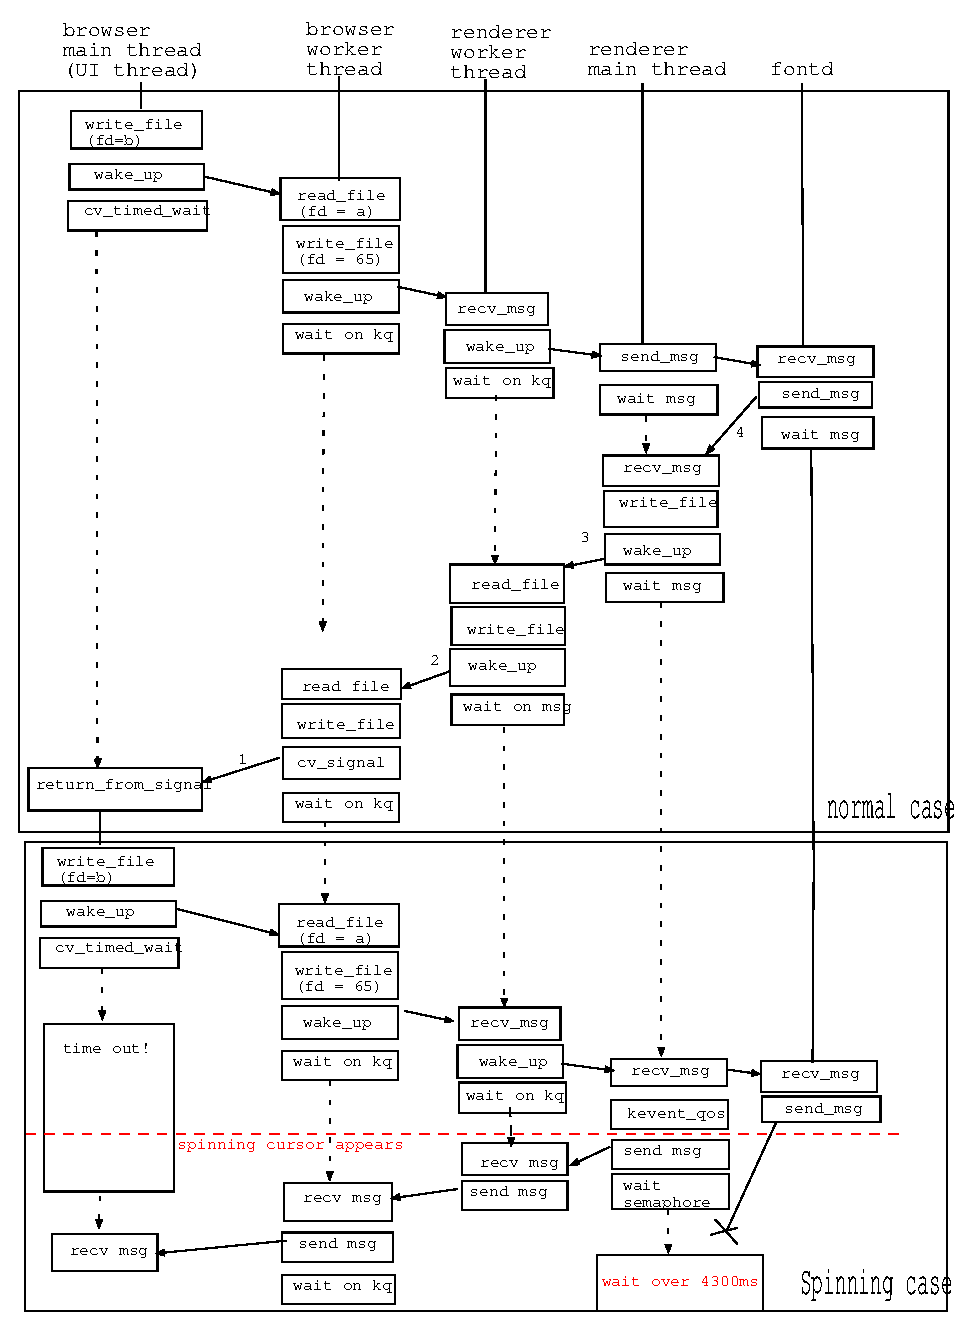
\includegraphics[width=0.8\linewidth]{chromium_case_study.eps}
    \caption{Chromium case study.}
    \label{fig:chromium-trace}
\end{figure*}

Next she ran \xxx to find the event in the main thread of the browser process.
\xxx returned a \v{cv\_timed\_wait} event (Figure~\ref{fig:chromium-trace})
that blocked the main thread for a few seconds.  Inspection of the lightweight
call stack revealed that this wait happened within a call to
\v{TextInputClientMac::GetFirstRectForRange}.  Without knowing the
application's semantics, she could not understand this method.  Thus she ran
\xxx to compare the spinning case to a normal case.  \xxx searched in the main
thread of the browser process for vertexes similar to this wait waiting
vertexes (contain \v{write\_file, cv\_timed\_wait} in this case) similar to
this wait, found three, and confirmed with the user which one she wanted.

\xxx then found the normal-case wake-up path shown in the figure, which
connects five threads.  The browser main thread was signaled by a browser
worker thread as shown in step \textcircled{1} of backward slicing in Figure
\ref{fig:chromium-trace}, which in turn \v{read\_file} in step \textcircled{2}
for IPC from a worker thread of \v{renderer}, the daemon for rendering screens.
The \v{renderer} worker thread is woken up by the \v{renderer} main thread to
\v{read\_file} \textcircled{3}, which in turn \v{recv\_msg} \textcircled{4}
from \v{fontd}, the font service daemon.  From this path, we could guess that
\v{GetFirstRectForRange} was for the browser to understand the bounding box of
the search string.  \xxx further compared the wake-up path with the spinning
case, and returned the \v{wait\_semaphore} event in the \v{renderer} main
thread, the culprit that delayed waking up the browser main thread over 4
seconds.

What caused the wait in the \v{renderer} main thread though?  She thus
continued diagnosis and recursively applied \xxx to the wait in \v{renderer},
and got the wake-up path shown in the figure for this wait.  Inspection reveal
that the \v{renderer} requested the browser's help to render Javascript and was
waiting for a reply.  At this point, a circular wait formed because the browser
was waiting for the \v{renderer} to return the string bounding box and the
\v{renderer} was waiting for the browser to help render Javascript.  This
circular wait was broken by a timeout in the browser main thread (the
\v{cv\_timed\_wait} timeout was 1,500 ms).  While the system was able to make
progress, the next key press caused the spinning cursor to display for another
1,500 ms.  The timeout essentially converted a deadlock into a livelock.

\subsection{Limitations}

\xxx is designed to support interactive debugging of performance issues.  To
incrementally obtain more fine-grained event traces, it needs to rerun an
application to reproduce a performance issue.  Thus, if the issue is difficult
to reproduce, we have to rely on the log collected by the lightweight
system-wide tracing for debugging, and lose the benefits of interactivity.
Fortunately, a performance issue that almost never reproduces is probably not
as annoying as one that occurs frequently.

We implemented \xxx in the closed-source MacOS which presents a harsh test for
\xxx, but we have not ported \xxx to other operating systems yet.  It is
possible that the ideas and techniques do not generalize to other operating
systems.  However, modern operating systems share many similarities, and good
ideas tend to flow both ways, so we are hopeful that the ideas in \xxx are
generally applicable.  Similarly, the applications and performance issues used
in our evaluation may be non-representative.
